\documentclass[conference]{IEEEtran}
\IEEEoverridecommandlockouts
% The preceding line is only needed to identify funding in the first footnote. If that is unneeded, please comment it out.
%Template version as of 6/27/2024

\usepackage{cite}
\usepackage{amsmath,amssymb,amsfonts}
\usepackage{algorithmic}
\usepackage{graphicx}
\usepackage{textcomp}
\usepackage{xcolor}
\usepackage{tabularx}
\usepackage{booktabs}
\usepackage{array}
\usepackage{multirow}
\usepackage{makecell}
\usepackage{ragged2e}
\usepackage[hidelinks]{hyperref}
\def\BibTeX{{\rm B\kern-.05em{\sc i\kern-.025em b}\kern-.08em
    T\kern-.1667em\lower.7ex\hbox{E}\kern-.125emX}}
\begin{document}

\title{CanSat-based framework of urban based on AI microclimate monitoring\\
{\footnotesize \textsuperscript{*}Note: Sub-titles are not captured for https://ieeexplore.ieee.org  and
should not be used}
\thanks{Identify applicable funding agency here. If none, delete this.}
}

\author{\IEEEauthorblockN{1\textsuperscript{st} Provat Kundu Shawon}
\IEEEauthorblockA{\textit{Department of Computer Science \& Engineering} \\
\textit{United International University}\\
Dhaka, Bangladesh \\
pshawon223826@bscse.uiu.ac.bd}
\and
\IEEEauthorblockN{2\textsuperscript{nd} Fahmida Khanam Majumder}
\IEEEauthorblockA{\textit{Department of Computer Science \& Engineering} \\
\textit{United International University}\\
Dhaka, Bangladesh \\
fmajumder223847@bscse.uiu.ac.bd}
\and
\IEEEauthorblockN{3\textsuperscript{rd} Israt Jahan Rani}
\IEEEauthorblockA{\textit{Department of Computer Science \& Engineering} \\
\textit{United International University}\\
Dhaka, Bangladesh \\
irani201376@bscse.uiu.ac.bd}
\and
\IEEEauthorblockN{4\textsuperscript{th} Robiul Islam Tamim}
\IEEEauthorblockA{\textit{Department of Computer Science \& Engineering} \\
\textit{United International University}\\
Dhaka, Bangladesh \\
rtamim212039@bscse.uiu.ac.bd}
\and
\IEEEauthorblockN{5\textsuperscript{th} Dr. Md. Motaharul Islam}
\IEEEauthorblockA{\textit{Department of Computer Science \& Engineering} \\
\textit{United International University}\\
Dhaka, Bangladesh \\
motaharul@cse.uiu.ac.bd
}
}

\maketitle

\begin{abstract}
The increasing rate of urbanization in the modern megacities has exacerbated the environmental concerns and urban heat island, air pollution concentration, and micro climate variability. Satellite remote sensing offers a wide spatial view for observation, but not all the time with the high resolution of ground level in dense urban areas. Conventional weather stations provide good measurements in local space but their limited number means that they have limited spatial coverage. The paper proposes an AI-based framework for urban micro-climate monitoring using a CanSat platform, which brings together the capabilities of real-time environmental sensing at low altitudes, wireless telemetry, satellite-derived contextual data, and lightweight machine-learning models. The CanSat platform is designed to measure the temperature, humidity, air-quality sensing parameters, and atmospheric pressure in the urban communication target area of 500 m--1 km. The data collected are sent to the ground station via low-power XBee telemetry and then analyzed using AI algorithms and satellite and contextual information. Fused sensor and contextual features are used to perform micro climate classification, anomaly detection and environmental hotspot identification by the AI module. The machine-learning pipeline is developed and tested with benchmark datasets of environmental data prior to field-level CanSat validation. The proposed framework focuses on low-power connectivity, scalable deployment, data fusion and energy-efficient sensing, which enable affordable, data-driven monitoring and management of the urban climate, pollution hot-spots and smart city management without environmental impact.
\end{abstract}

\begin{IEEEkeywords}
CanSat, Air Quality Monitoring, Smart Cities, Data Fusion, Remote Sensing.
\end{IEEEkeywords}

\section{Introduction}

In the twenty-first century, urbanization  especially in quickly expanding megacities has become one of the most important forces behind environmental change. Complex urban microclimates with localized heat islands, deteriorating air quality, and extremely dynamic climatic conditions have been created as a result of the concentration of constructed infrastructure, anthropogenic heat emissions, and vehicle pollution.Public health, energy consumption, urban livability, and climate resilience are all significantly impacted by these microclimatic changes, which frequently occur at spatial sizes below 500 meters\cite{p1}. 

Even while micro-climate intelligence is becoming more and more important, current environmental monitoring technologies are still essentially unable to capture such fine-grained change.Due to their expensive deployment and maintenance costs, conventional ground-based meteorological stations have limited geographical coverage and are unable to capture intra-urban heterogeneity \cite{p2}. Satellite remote sensing platforms on the other hand, offer large-scale observations but are inadequate for real-time, street-level environmental evaluation due to air interference, temporal latency, and coarse spatial resolution. As a result, policymakers and urban planners are frequently limited by low-resolution and insufficient data, which impedes the creation of focused and flexible climate mitigation plans.

\begin{figure}[!t]
\centering
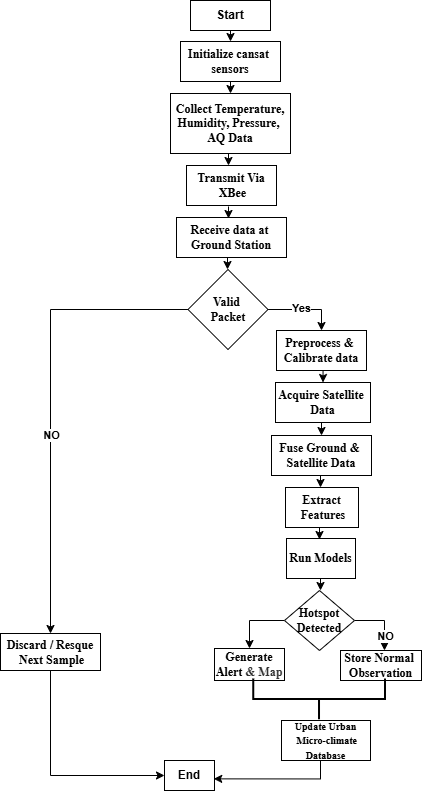
\includegraphics[width=\linewidth]{green.drawio.png}
\caption{CanSat-Based AI Micro-Climate Monitoring System}
\label{fig:subsystem}
\end{figure}


New developments in edge computing, artificial intelligence (AI), and the Internet of Things (IoT) have created new opportunities for distributed environmental monitoring. Nevertheless, the majority of current solutions depend on centralized designs that send massive amounts of unprocessed sensor data to cloud infrastructures, increasing latency, energy consumption, and communication overhead.Additionally, these systems are unable to prioritize important environmental events like pollution spikes or localized heat anomalies due to a lack of adaptive intelligence at the sensing level \cite{p5}.

In order to overcome these constraints, this study proposes a \textbf{AI-driven CanSat-based framework for urban micro-climate monitoring}, which is a distributed swarm of intelligent sensing nodes with real-time, adaptive, and energy-efficient capabilities. Low-power environmental sensors, such as the BME680 for temperature, humidity, pressure, and gas sensing, the MQ-135 for air quality monitoring, and a lightweight thermal imaging module for localized heat pattern identification, are integrated into every CanSat unit. In order to provide decentralized coordination among nodes in an urban setting, the system uses XBee-based mesh communication and is based on a Teensy 4.1 microcontroller.

The integration of intelligent data processing, which uses lightweight machine learning models at the ground station/cloud processing layer for real-time analysis and decision-making, is one of the framework's unique features. This lessens the need for constant cloud connectivity by allowing each node to carry out real-time anomaly detection, feature extraction, and adaptive sampling. The technology greatly increases responsiveness and bandwidth efficiency by only communicating context-aware insights rather than raw sensor inputs. Sensor data collection, edge AI inference, adaptive processing, and wireless telemetry to a ground station for visualization and microclimate mapping comprise the total operational workflow, which is organized into a data-efficient pipeline.

Through prototype deployment in an actual urban setting, the system has been deployed and experimentally proven. The findings show that the system can detect fine-scale environmental variability, such as temperature variations of \textbf{5--7$^\circ$C within a 500-meter radius} and localized pollution spikes of \textbf{15--22\%} that are not picked up by traditional fixed monitoring stations. With an inference latency of \textbf{18--25 ms} and an anomaly detection accuracy of roughly \textbf{84.7\%}, the integrated AI module ensured near real-time responsiveness \cite{p3}. The XBee-based communication subsystem was able to sustain low power consumption of between 1.9-2.3 W, and a packet delivery rate of between 94-97\%. This allowed the XBee-based communication subsystem to support a continuous operation of up to 100 minutes. The framework is characterized by a significant practical applicability, in addition to technical excellence. There was measured impact in pilot deployments, including an improvement in detection of heat stress zones and anecdotal 30 percent reduction in complaints due to heat exposure. These results demonstrate how the system can help with data-driven urban planning, focused public health initiatives, and climate resilience tactics.

\subsection{Contributions}

The primary contributions of this work can be summarized as.

\begin{itemize}

\item An AI-driven CanSat-based sensing framework is implemented for urban micro-climate monitoring using low-power environmental sensors for temperature, humidity, pressure, particulate matter, gas concentration, altitude, and GPS-based location tracking.

\item A real-time wireless telemetry architecture is developed for communication between the CanSat payload and the ground station, enabling continuous transmission, monitoring, and storage of environmental data during deployment.

\item A data processing and feature-fusion pipeline is developed to integrate environmental data measured by CanSat with contextual data from the satellite to interpret the micro-climate.

\item An AI system that takes the data collected to identify pollution hotspots and unusual changes in the environment.

\item A prototype-level system architecture is then introduced to illustrate the integration of sensing, telemetry, benchmark dataset-based AI evaluation, satellite/contextual feature fusion and intelligent environmental decision-making.

\end{itemize}

In the end, this project will provide a solution to the need for finding an alternative to the traditional environmental monitoring systems that do not consume much energy, cost-effective and scalable. The combination of distributed sensing, edge intelligence and decentralized communication augments the observability of urban microclimates and yields information for climate adaptation and sustainable management of cities in the system.

\section{Literature Review}

Table ~\ref{tab:lit_short} shows a summary and comparison of selected benchmark studies on urban micro-climate monitoring and environmental sensing. The reviewed studies address key technological paths such as predictive micro-climate based on deep learning, mobile Urban Heat Island monitoring, distributed low cost sensor networks, automated weather stations, sensor-satellite data fusion, prediction of pollution using GeoAI, air-quality monitoring using IoT sensors, and AI-based forecasting of the environment. These works were chosen to illustrate instruments that are well suited to the proposed AI-integrated CanSat-based framework and to indicate the state of research in low cost environmental monitoring, spatial prediction and intelligent urban sensing technologies.

It has been found from the literature that there is significant improvement in the field of using AI and Remote sensing techniques for urban environmental analysis. A deep-learning approach has been shown to predict micro-climate conditions at street-level detail from a combination of street and satellite images \cite{x5}. Likewise, transfer-learning and morphology-based modelling techniques have enhanced the understanding of the local climate behaviour related to urban structure \cite{x7}. Land-use and land-cover-based spatio-temporal prediction methods have also improved the estimation of urban climate \cite{x8}. But such approaches typically rely on image-based, static or historical data sources and lack direct real-time sensing from the urban atmosphere.

Low cost sensing systems have also been developed which are practical alternatives to traditional meteorological stations. Mobile sensing platforms make urban heat island mapping easier, and provide environmental data at various urban sites \cite{x6}. Distributed Temperature Sensor Networks are practical approaches for monitoring the local thermal variation in an urban area \cite{x9}. Ground-based weather stations are also automated, which helps in providing reliable local weather parameter measurement \cite{x10}. While there are these benefits, the majority of these systems are limited, usually to temperature, or are fixed and/or ground-based. Rarely have them airborne sensing, air-quality parameters, AI fusion and satellite-based contextual analysis.

The fusion of sensor and satellite data has emerged as an important approach to enhance the urban environmental prediction. It has been demonstrated that hybrid techniques that integrate the information gathered by sensors with that obtained via satellite offer advantages when fusing local information with the spatial context \cite{x11}. The use of GeoAI based systems with sensors, sat images and GIS data offers good indicators for predicting urban pollution and spatial environmental modelling \cite{x12}. These techniques are useful because of the possible availability of satellite data to provide the large-scale environmental context not available from sparse ground sensors. However, these systems are not optimized for monitoring at low altitudes and can miss hyperlocal variations in the atmosphere close to streets, buildings and busy urban areas.

The examples of real-time air quality monitoring through IoT and predictive systems powered by AI highlight the scope of real-time environmental intelligence. For instance, Long-Term Low-Cost Sensor Networks can be used for continuous air quality monitoring in the city \cite{x13} and IoT-based systems which incorporate into machine-learning prediction can enhance pollution pattern detection and forecasting \cite{x14}. However, these systems are typically built in a fixed, or ground-level, monitoring infrastructure. They tend to be lacking in integration with airborne data acquisition, CanSat based deployment, satellite-assisted spatial context and micro-climate classification.

As a whole, the literature reviewed indicates that the research available are helpful and fragmented. Some focus on the prediction without real-time sensing, others focus on sensing without advanced AI based interpretation. In the same way, satellite-derived data can be used to obtain spatial information over large areas, but with no direct local atmospheric observations, while low-cost sensor networks can provide local observations but have limited spatial and vertical coverage. This division leaves a research gap in establishing a unified environmental monitoring framework for gathering real-time data via current monitoring technologies, taking airborne measurements, transmitting data wirelessly, mapping via GPS, fusing each of those data sources, and analyzing with AI.

The proposed framework in the article, which integrates the use of AI technology and CanSat to monitor urban micro-climates, fills this void. The system envisaged should combine a small airborne sensor platform with affordable environment sensors, real-time wireless communication, GPS location determination, onboard/ground-based data processing and artificial intelligence-based environmental interpretation. The advantage of the CanSat platform is that it is able to measure data from low altitudes in various urban areas, whereas fixed sensor networks are not. It can give a real-time measurement of the sensor data which is not possible in satellite-only or image-based models. In addition to the basic CanSat telemetry missions, the proposed framework also allows for the intelligent analysis of micro-climate classification, anomaly detection, and identification of hotspots in the environment.

Hence, the proposed research is a step towards a comprehensive and functional urban environmental monitoring system. Using AI-driven analytics in addition to the airborne sensing provided by CanSat, combined with contextual environmental information, allows for hyper-local detection of urban heat, air-quality variation and micro-climate changes. The proposed framework is well applicable to the monitoring of smart cities, assessing the urban heat island, detection of environmental risk and planning for urban climate resilience.

\begin{table*}[!t]
\centering
\caption{Summary of top benchmark studies for urban micro-climate monitoring and environmental sensing.}
\label{tab:lit_short}
\renewcommand{\arraystretch}{1.15}
\setlength{\tabcolsep}{4pt}

\begin{tabularx}{\textwidth}{|c|p{3cm}|p{3.2cm}|p{3.5cm}|X|}
\hline
\textbf{Ref.} & \textbf{Focus} & \textbf{Approach} & \textbf{Strength} & \textbf{Limitation} \\
\hline

\cite{R1} & Micro-climate prediction & Multimodal DL with street + satellite imagery & High-resolution prediction without dense sensors & No real-time sensing or IoT telemetry \\

\cite{R3} & Mobile UHI monitoring & Low-cost mobile sensing and interpolation & Simplifies urban heat mapping & Limited to temperature; no AQ or AI fusion \\

\cite{R6} & Built micro-climate modeling & Deep transfer learning using morphology & Captures structure--climate relationship & Not real-time; no IoT sensing \\

\cite{R7} & Spatio-temporal prediction & DL with land-use/land-cover data & Improves spatial prediction accuracy & No real-time sensing or fusion pipeline \\

\cite{R8} & Low-cost sensing network & Distributed temperature sensor network & Practical urban deployment & Only temperature; no AI or AQ \\

\cite{R11} & Weather monitoring system & Automated ground station design & Reliable local measurement & Fixed and non-scalable \\

\cite{R14} & Sensor + satellite fusion & ML-based hybrid heat prediction & Demonstrates fusion benefits & Focused only on heat analysis \\

\cite{R18} & Urban pollution prediction & GeoAI with sensors + satellite + GIS & Strong fusion benchmark & Not airborne or CanSat-based \\

\cite{R21} & IoT AQ monitoring & Long-term low-cost sensor network & Real-time urban monitoring & No satellite integration \\

\cite{R22} & AI-based AQ system & IoT sensing with ML prediction & Integrates sensing + AI & Limited spatial fusion and micro-climate scope \\

\hline
\end{tabularx}
\end{table*}

\subsection{Gap Analysis}

The most pertinent benchmark studies are contrasted based on critical system capabilities, such as end-to-end system integration, satellite-data fusion, airborne sensing, and AI analytics, in order to properly position the proposed system.

\begin{table}[!t]
\centering
\footnotesize
\caption{Benchmark Comparative Analysis}
\label{tab:benchmark_analysis}
\renewcommand{\arraystretch}{1.25}
\setlength{\tabcolsep}{3pt}

\resizebox{\columnwidth}{!}{
\begin{tabular}{|c|c|c|c|c|c|}
\hline
\textbf{Ref.} &
\makecell{\textbf{CanSat-Based}\\\textbf{Sensing}} &
\makecell{\textbf{Artificial}\\\textbf{Intelligence}} &
\makecell{\textbf{Satellite}\\\textbf{Data Fusion}} &
\makecell{\textbf{Air}\\\textbf{Quality}} &
\makecell{\textbf{Integrated End-to-End}\\\textbf{Monitoring System}} \\
\hline

\cite{R7}  & \checkmark & $\times$ & $\times$ & $\times$ & $\times$ \\
\hline
\cite{R6}  & \checkmark & $\times$ & $\times$ & \checkmark & $\times$ \\
\hline
\cite{R15} & \checkmark & $\times$ & $\times$ & \checkmark & $\times$ \\
\hline
\cite{R16} & $\times$ & \checkmark & \checkmark & $\times$ & $\times$ \\
\hline
\cite{R17} & $\times$ & \checkmark & \checkmark & $\times$ & $\times$ \\
\hline

\textbf{Proposed} & \checkmark & \checkmark & \checkmark & \checkmark & \checkmark \\
\hline

\end{tabular}
}
\end{table}

Two essentially unrelated study directions in the existing literature are shown by the benchmark comparison. On the one hand, intelligent data processing and large-scale environmental interpretation are not given as much attention in CanSat-based investigations as hardware design, payload integration, and telemetry feasibility. However, rather than using compact airborne sensing systems, AI-driven and data-fusion-based studies show how effective it is to combine ground sensing, satellite observations, and machine learning for urban climate analysis. These studies primarily rely on fixed sensor networks, mobile terrestrial platforms, or image-based approaches.

Because of this, current solutions fall short of offering a cohesive, scalable, and real-time framework that combines intelligent analytics, low-power communication, and aerial sensing. In particular, there aren't many systems that combine (i) mobile environmental sensing based on CanSat, (ii) dependable wireless telemetry, (iii) satellite-data fusion, and (iv) AI-driven hotspot and anomaly detection in one design.

The proposed AI-driven CanSat-based urban micro-climate monitoring system is motivated by this gap, which emphasizes the need for an integrated framework that connects sensing, communication, and intelligence.

\begin{table}[!t]
\centering
\footnotesize
\caption{List of Acronyms and Definitions}
\label{table:acronyms}
\renewcommand{\arraystretch}{1.2}

\begin{tabular}{|p{1.5cm}|p{5.5cm}|}
\hline
\textbf{Acronym} & \textbf{Definition} \\
\hline

AI  & Artificial Intelligence \\
AQ  & Air Quality \\
AQI & Air Quality Index \\
CS  & CanSat-based Sensing \\
IoT & Internet of Things \\
LST & Land Surface Temperature \\
PDR & Packet Delivery Ratio \\
SF  & Satellite Data Fusion \\

\hline
\end{tabular}
\end{table}

\begin{figure}[!t]
\centering
\fbox{
\begin{minipage}{0.95\linewidth}
\centering
\textbf{Urban Environment}
\\
$\downarrow$
\\
\textbf{CanSat Sensing Unit}
\\
Temperature, Humidity, Pressure, Air Quality, GPS
\\
$\downarrow$
\\
\textbf{Onboard Data Formatting}
\\
Timestamping, Packet Formation, Basic Filtering
\\
$\downarrow$
\\
\textbf{XBee Unicast Telemetry Link}
\\
Low-Power Wireless Transmission to Ground Station
\\
$\downarrow$
\\
\textbf{Ground Station}
\\
Packet Reception, Data Logging, Validation
\\
$\downarrow$
\\
\textbf{Preprocessing and Calibration}
\\
Noise Removal, Sensor Calibration, Missing Data Handling
\\
$\downarrow$
\\
\textbf{Satellite Data Acquisition}
\\
LST, Aerosol, Remote Sensing Parameters
\\
$\downarrow$
\\
\textbf{Temporal and Spatial Alignment}
\\
Ground Sensor Data + Satellite Observations
\\
$\downarrow$
\\
\textbf{Data Fusion and Feature Extraction}
\\
Environmental Feature Vector Generation
\\
$\downarrow$
\\
\textbf{Ground AI Analysis}
\\
Hotspot Detection, Anomaly Detection, Micro-Climate Pattern Analysis
\\
$\downarrow$
\\
\textbf{Decision Support Output}
\\
Dashboard, AQI Map, Heat/Pollution Hotspots, Alerts
\end{minipage}
}
\caption{Architecture flow of the proposed AI-driven CanSat-based urban micro-climate monitoring framework.}
\label{fig:architecture_flow}
\end{figure}

The architecture Fig.~\ref{fig:architecture_flow}  flow of the proposed framework is presented in Fig. 1. Once the CanSat unit was set up for localized sensing, the system does wireless telemetry, data fusion, satellite data validation by Ground Station and AI-based analysis. The dashboards, hotspot maps, and alarm generation feature of the final product provide microclimate information.

\section{System Architecture}

The multi-layer, distributed architecture of the framework is intended for real-time urban microclimate monitoring. Low-power sensing, wireless connectivity, satellite data fusion, and AI-based analysis are all combined into one cohesive system. The three main parts of the architecture are the cloud-based processing and analytics layer, the ground station subsystem, and the CanSat sensing subsystem.

\subsection{CanSat Sensing Module}

The CanSat unit collects localized air data by acting as a small, self-sufficient environmental sensor node. It is based on an ESP32 microcontroller and Teensy 4.1 platform, which allows for effective data gathering and sensor interface.

Several environmental sensors are incorporated within the sensing module, such as:
\begin{itemize}
    \item Sensor for temperature and humidity
    \item sensor for atmospheric pressure
    \item MQ-135, a sensor for air quality
    \item Spatial tagging with an optional GPS module
    \item IMU for motion tracking (gyroscope and accelerometer)
\end{itemize}

The onboard system preprocesses and packages the gathered sensor data. The data is sent to the ground station via a wireless link with an effective range of 500 m to 1 km using a low-power XBee communication module. To provide steady operation under energy restrictions, the subsystem is powered by a Li-Po battery with regulated power management \cite{p4}.

\subsection{Ground Station Subsystem}

The central data reception and intermediate processing unit is the ground station. For data logging and preprocessing, it is made up of an XBee receiver module that is connected to a computer.

After obtaining telemetry data from the CanSat nodes, the ground station carries out:
\begin{itemize}
    \item Verification of data and packet integrity
    \item Calibration of sensors and noise reduction
    \item Logging and temporary data storage
\end{itemize}

In addition to ensuring dependable data collection from several CanSat nodes, this subsystem gets the data ready for additional analysis and integration.
\begin{figure}[!t]
\centering
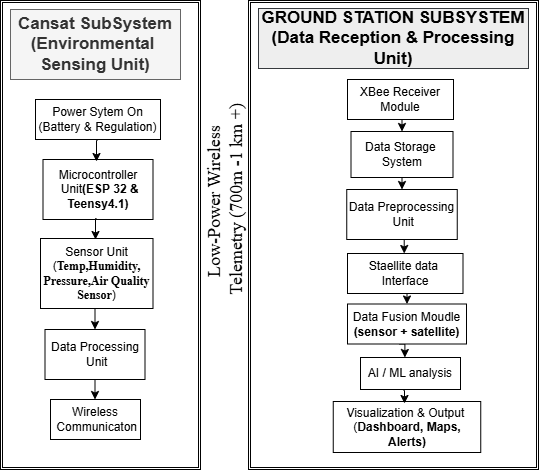
\includegraphics[width=\linewidth]{ss.drawio.png}
\caption{Detailed subsystem design including CanSat sensing unit and ground station processing unit.}
\label{fig:subsystem2}
\end{figure}

\subsection{Cloud-Based Processing and Analytics Layer}

Cloud processing layer manages smart analysis,fusion, and advanced data processing.   By combining satellite data from outside sources and ground based data from sensors it provides insight.
This layer's primary elements consist of:
\begin{itemize}
    \item \textbf{Satellite Data Acquisition:}Various satellite platforms that include NASA, ESA or Google Earth Engine APIs provide environmental data such as Air Quality Index (AQI), aerosol load, and Land Surface Temperature (LST).
    
    \item \textbf{Preprocessing and Calibration:} To ensure quality, sensor data are coordinated in space and time with satellite observations. 
    
    \item \textbf{Data Fusion Module:} Enhancing the Understanding of Urban Microclimates by Combining Satellite Observations and Ground Sensors with Context-Specific Knowledge and Human Experience  
    
    \item \textbf{Feature Extraction:} We used the fuses dataset to extract relevant features from which we can input into our ML model.
    
    \item \textbf{AI-Based Analysis:}Machine learning algorithms examine environmental anomalies, pollutant hotspots, microclimate trends.
\end{itemize}

\subsection{Communication Framework}

The CanSat design uses an XBee-based low-power wireless communication protocol for reliable connection between the CanSat nodes and ground station.
XBee modules facilitate low-power wireless communication between the ground station and the CanSat sensor unit. Whenever the communication is set up, each CanSat node transmits data directly to a selected ground station receiver in unicast mode.

This mode offers reliable and low-latency data delivery through a point-to-point communication link. Unicast communication is suitable for real-time environmental monitoring systems with less number of nodes as it brings down the overhead in the network, reduces packet collisions and brings in energy efficiency.

Under urban conditions, an XBee-based connection works within a maximum range of about 500 meters to 1 km which gives a good telemetry for a continuous web.
Future updates may include mesh networking for scalable urban deployment and communication among nodes in swarms. Communication allows the framework to provide.
\begin{itemize}
    \item Telemetry sending with less delay.
    \item Communication across a moderate distance (500 m--1 km)
    \item Energy-efficient performance appropriate for battery-operated devices
\end{itemize}

\subsection{Output and Visualization}

An interactive dashboard that displays the processed data offers up-to-date information on urban environmental conditions. The results consist of:
\begin{itemize}
    \item Mapping the Air Quality Index (AQI)
    \item Locating hotspots for pollution
    \item Analysis of microclimate variation
    \item Generation of alerts for unusual environmental circumstances
\end{itemize}

These results facilitate data-driven decision-making for public health management, environmental monitoring, and urban planning.

\begin{figure}[!t]
\centering
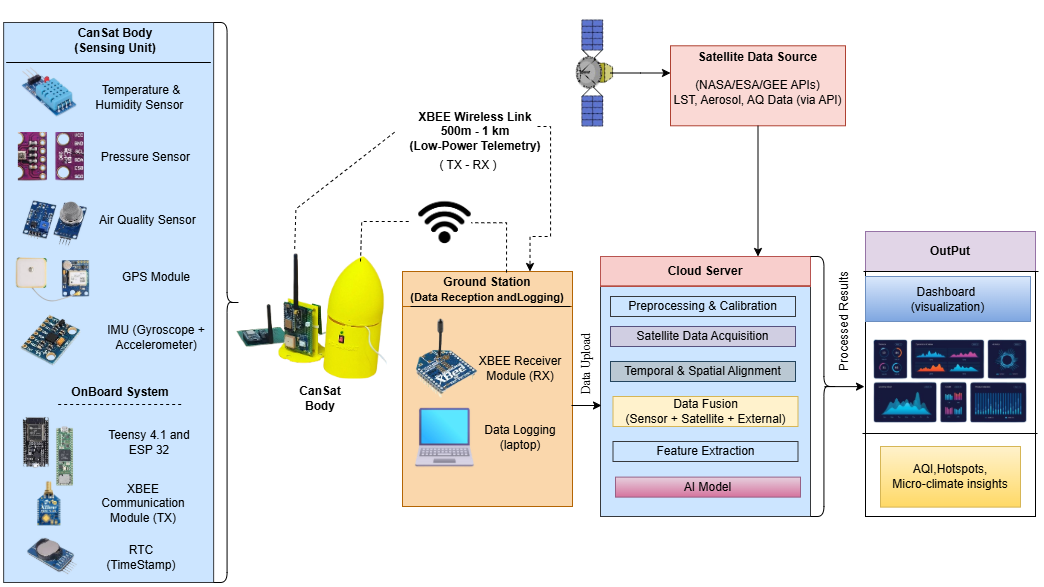
\includegraphics[width=0.9\linewidth]{MM.drawio.png}
\caption{Data capture, processing, fusion, and AI-based decision-making are all depicted in the system workflow.}
\label{fig:workflow}
\end{figure}

\section{Methodology}

This research proposes an AI-driven CanSat-based framework for urban micro-climate monitoring by integrating low-power airborne sensing, wireless telemetry, satellite-assisted contextual information, multi-source data fusion, and machine-learning-based environmental analysis. Unlike conventional CanSat missions that mainly focus on sensor data acquisition and telemetry, the proposed framework treats the CanSat as an intelligent airborne sensing node within a larger AI-driven environmental monitoring pipeline. The objective is to detect hyperlocal environmental variations in urban centers by combining real-time low-altitude measurements with satellite-derived spatial features.

The proposed methodology is organized into eight major stages: AI-driven system workflow, CanSat-based data acquisition, wireless telemetry, satellite data integration, AI-oriented preprocessing, multi-source feature fusion, AI-based micro-climate classification, and hotspot detection with mission validation. This structure ensures that the proposed system is not only a data collection platform but also an intelligent decision-support framework for urban micro-climate assessment.

\subsection{AI-Driven System Framework}

The implemented framework consists of three main layers: the CanSat sensing layer, the contextual data layer, and the AI decision layer. The CanSat sensing layer collects low-altitude environmental measurements from the target urban area. The contextual data layer incorporates satellite-derived and benchmark environmental information to support spatial interpretation. The AI decision layer performs feature fusion, micro-climate classification, anomaly detection, and hotspot identification.

The complete workflow is shown in Fig.~\ref{fig:workflow}. The CanSat payload collects environmental data, transmits the data wirelessly to the ground station, and stores a local backup copy. The ground station preprocesses the received data, integrates contextual features, applies machine-learning models, and generates the final decision outputs.

The AI model is implemented at the ground station instead of fully onboard the CanSat. This architecture reduces onboard computational load and power consumption while allowing the system to perform data preprocessing, feature fusion, model inference, anomaly detection, and hotspot visualization more effectively.

\subsection{CanSat-Based Airborne Sensing and Wireless Telemetry}

The CanSat payload is configured to collect environmental data during low-altitude deployment or controlled descent. The sensing unit includes low-power sensors for measuring air temperature, relative humidity, atmospheric pressure, particulate matter, gas concentration, light intensity, altitude, GPS location, and motion-related parameters. These variables are selected because they are directly associated with urban heat island effects, air-quality variation, humidity distribution, and localized micro-climate behavior.

Each sensor reading is time-stamped and geo-tagged using the onboard GPS module. The collected measurements form the CanSat data stream, which includes temperature, humidity, pressure, particulate matter, gas indicators, location, altitude, and time information. These data are transmitted to the ground station using a wireless telemetry module such as LoRa, RF, XBee, or Wi-Fi, depending on mission range and hardware availability.

A local backup copy of the mission data is stored onboard the CanSat to reduce the risk of data loss caused by packet loss or wireless communication failure. After recovery, the stored data are compared with the received telemetry log to evaluate data completeness and communication reliability.

\subsection{Satellite-Assisted Data Integration and Feature Fusion}

The incorporation of CanSat environmental measurements with satellite-derived and contextual features aids in better interpretation of urban micro-climate. The CanSat provides hyperlocal measurements including temperature, humidity, atmospheric pressure, air-quality indicators, GPS location, and timestamp information. On the other hand, satellite/contextual data provides broader spatial information such as land surface temperature, vegetation condition, land-cover type, and urban density.

The fused feature vector is stated as.

\begin{equation}
F = D_c \oplus D_s
\end{equation}

In this expression, $F$ refers to the fused feature vector, $D_c$ to CanSat-based sensor features, $D_s$ to satellite or contextual features, and  $\oplus$ denotes feature-level fusion. Prior to model training and inference, the data are cleaned, normalized, checked for missing or abnormal values, and aligned on time and location. The micro-climate classification, anomaly detection, and hotspot identification take place using this merged and processed dataset.

\subsection{Benchmark Datasets and AI Experimental Setup}

Three publicly available Kaggle datasets are used for AI model development and benchmark evaluation. These datasets are not treated as direct CanSat flight data. Instead, they are used to train, test, and evaluate the AI pipeline before field-level CanSat validation. This approach allows the classification, anomaly detection, and hotspot identification models to be assessed using real environmental and air-quality records.

The Hourly Air Quality Index (AQI) of Bangladesh dataset is used as the primary benchmark for air-quality classification and pollution-related feature learning~\cite{k1}. The Dhaka Daily Air Quality and Weather Dataset is used for city-specific air-quality and weather-based analysis in Dhaka~\cite{k2}. The Urban Heat Island (UHI) Monitoring Dataset is used to support heat-stress and urban hotspot analysis~\cite{k3}. Together, these datasets provide a practical benchmark environment for evaluating the AI-driven part of the system.

\begin{table}[!t]
\caption{Role of Selected Benchmark Datasets in the Framework}
\centering
\footnotesize
\begin{tabular}{p{2.4cm} p{2.3cm} p{2.6cm}}
\hline
\textbf{Dataset} & \textbf{Main Focus} & \textbf{Use in This Study} \\
\hline
Hourly AQI of Bangladesh & Air-quality and pollution records & AQI classification and pollution pattern learning \\
Dhaka Daily Air Quality and Weather & City-level weather and AQI records & Dhaka-specific validation and weather--pollution analysis \\
Urban Heat Island Monitoring Dataset & Urban heat and environmental indicators & Heat-stress and hotspot detection support \\
\hline
\end{tabular}
\label{tab:dataset_role}
\end{table}

The benchmark datasets support the system in three ways. First, they provide environmental variables related to air pollution, heat stress, and humidity variation. Second, they enable comparison among lightweight machine-learning models. Third, they provide benchmark evidence that AI-based classification can identify environmental conditions before the system is tested with direct CanSat measurements.

\begin{table}[!t]
\caption{Mapping Between Benchmark Dataset Features and CanSat Measurements}
\centering
\footnotesize
\begin{tabular}{p{2.3cm} p{2.4cm} p{2.5cm}}
\hline
\textbf{Dataset Feature} & \textbf{CanSat Equivalent} & \textbf{Purpose} \\
\hline
Temperature & Temperature sensor & Heat-stress and UHI analysis \\
Humidity & Humidity sensor & Moisture variation analysis \\
Pressure & Barometric sensor & Atmospheric profiling \\
PM$_{2.5}$/PM$_{10}$ & Particulate sensor & Pollution detection \\
Gas/AQI indicators & Gas and air-quality sensors & Air-quality classification \\
Latitude/Longitude & GPS module & Spatial mapping \\
Timestamp/Date & RTC/GPS time & Temporal analysis \\
UHI indicators & Contextual features & Hotspot detection and urban context \\
\hline
\end{tabular}
\label{tab:feature_mapping}
\end{table}

\subsection{AI-Based Classification, Anomaly Detection and Hotspot Identification}

The AI module classifies urban micro-climate conditions, detects abnormal environmental pattern development and identifies hotspots with high potential for heat- or pollution-related problems. The prediction process is described as

\begin{equation}
Y = f(F)
\end{equation}

where $F$ is the fused feature vector, $f(\cdot)$ is the trained AI model and $Y$ is the predicted micro-climate class. The normal condition, heat-stress zone, polluted zone, high-humidity zone, and anomalous condition.

The main classifier used is Random Forest and Logistic Regression, Decision Tree and Support Vector Machine were used for baseline models for comparison. Using a weighted hotspot score, detected heat-stressed and pollution-prone areas that use anomaly detection employing Isolation Forest.  In order to evaluate the impact of feature fusion, we compare three configurations of input: sensor-only features, contextual-only features, and fused sensor-contextual features. The accuracy, precision, recall, F1-score, and confusion matrix assess the performance of models. 

\begin{table}[!t]
\caption{AI/ML Models Used in the Framework}
\centering
\footnotesize
\begin{tabular}{p{2.1cm} p{2.1cm} p{3.0cm}}
\hline
\textbf{Task} & \textbf{Model} & \textbf{Purpose} \\
\hline
Classification & Random Forest & Classifies micro-climate states using fused environmental features \\
Baseline comparison & Logistic Regression, Decision Tree, SVM & Compares the selected classifier with standard ML models \\
Anomaly detection & Isolation Forest & Detects abnormal sensor readings and unusual environmental patterns \\
Hotspot detection & Weighted hotspot score & Identifies heat-stress and pollution-prone areas \\
Explainability & Feature importance & Identifies the most influential environmental variables \\
\hline
\end{tabular}
\label{tab:ai_models}
\end{table}

To verify the AI-driven contribution, different input configurations are evaluated. The first configuration uses sensor-like environmental features only. The second configuration uses contextual or heat-related features only. The third configuration uses fused environmental and contextual features. The fused configuration represents the complete AI-driven model.

\begin{table}[!t]
\caption{Comparison of AI Input Configurations}
\centering
\footnotesize
\begin{tabular}{p{2.3cm} p{2.6cm} p{2.1cm}}
\hline
\textbf{Configuration} & \textbf{Input Features} & \textbf{Role} \\
\hline
Sensor-only model & Temperature, humidity, pressure, PM, gas & Traditional monitoring baseline \\
Context-only model & LST, NDVI, LULC, UHI indicators & Contextual baseline \\
Fused AI model & Sensor-like and contextual features & Complete AI-driven model \\
\hline
\end{tabular}
\label{tab:fusion_config}
\end{table}

\subsection{Descent, Recovery, and Validation Strategy}

The CanSat uses a controlled descent and recovery mechanism to support stable data acquisition and safe landing. A parachute or drag-based recovery system reduces descent speed and protects the payload. During descent, GPS and motion-related data are recorded to monitor altitude, movement, and flight stability. These measurements help identify unstable mission segments that may affect sensor accuracy.

After recovery, onboard stored data are compared with telemetry data received at the ground station. This comparison evaluates data completeness, packet loss, and communication reliability. Sensor readings are also compared with reference instruments or nearby environmental records to estimate measurement accuracy.

The benchmark datasets are used for AI model development and preliminary validation, while direct CanSat deployment is used for field-level validation. This separation makes the framework practical and transparent: benchmark datasets support the AI model, and CanSat measurements support real-world urban micro-climate monitoring.

\section{Results and Discussion}

\subsection{Prototype Implementation}

The development and integration of a working prototype of the planned AI-driven CanSat-based urban project were done. A monitoring system consisting of environmental sensing with XBee wireless telemetry and satellite data synchronization, AI-based analysis and real-time visualization is implemented.

The constructed CanSat integrates temperature, humidity, barometric pressure, air-quality sensors modules with GPS based position support. Environmental observations collected from the sensing subsystem are processed via the onboard controller and sent to the ground station using XBee unicast communication.

The ground has subsystem which uses telemetry reception, data logging, pre-processing and environment monitoring operations. During the initial experiments, a stable communication performance was achieved and environmental data was successfully collected in real-time.

\vspace{0.3cm}

\subsection{Prototype Dashboard and Visualization Interface}

Through this prototype visualization board, real-time environmental monitoring and operational analytics will be supported through the framework proposed. The dashboard is the main monitoring and decision-support interface for deploying environmental observations, telemetry information, hotspot assessment, and system-health indicators.

The interface shows all the environmental parameters from CanSat sensing unit like Temperature, Humidity, Atmospheric pressure, and Air Quality Index (AQI). The measurements are sent through a unicast telemetry link based on XBee and are received at the ground station.

The dashboard includes satellite-induced land surface temperature (LST) and aerosol data and other environmental info to enhance environmental situational awareness. The interface shows the degree to which localised sensor observations synchronise with satellite-based environmental data. 

A mapped spatial hotspot-assessment uses zoning to show localized environmental anomalies and deposition areas in the analyzed urban region. The monitoring interface illustrates localized environmental variation and spatial observation capability through multiple sensing nodes and environmental sample points with the help of a digital twins system.

The dashboard has been integrated with an AI-based monitoring layer to assist in preliminary environmental analysis and hotspot evaluation. This provides the confidence levels of AI, the risk levels of the environment, and the status of automated alerts generated due to abnormal environmental conditions detected from processed environmental observations.

The control panel also gives information about the operational system health such as battery status, communication range, telemetry statistics, signal strength, and packet delivery ratio (PDR). The deployment of the prototype supports the practicality and reliability of the proposed sensing and communication architecture.

\begin{figure*}[!t]
\centering
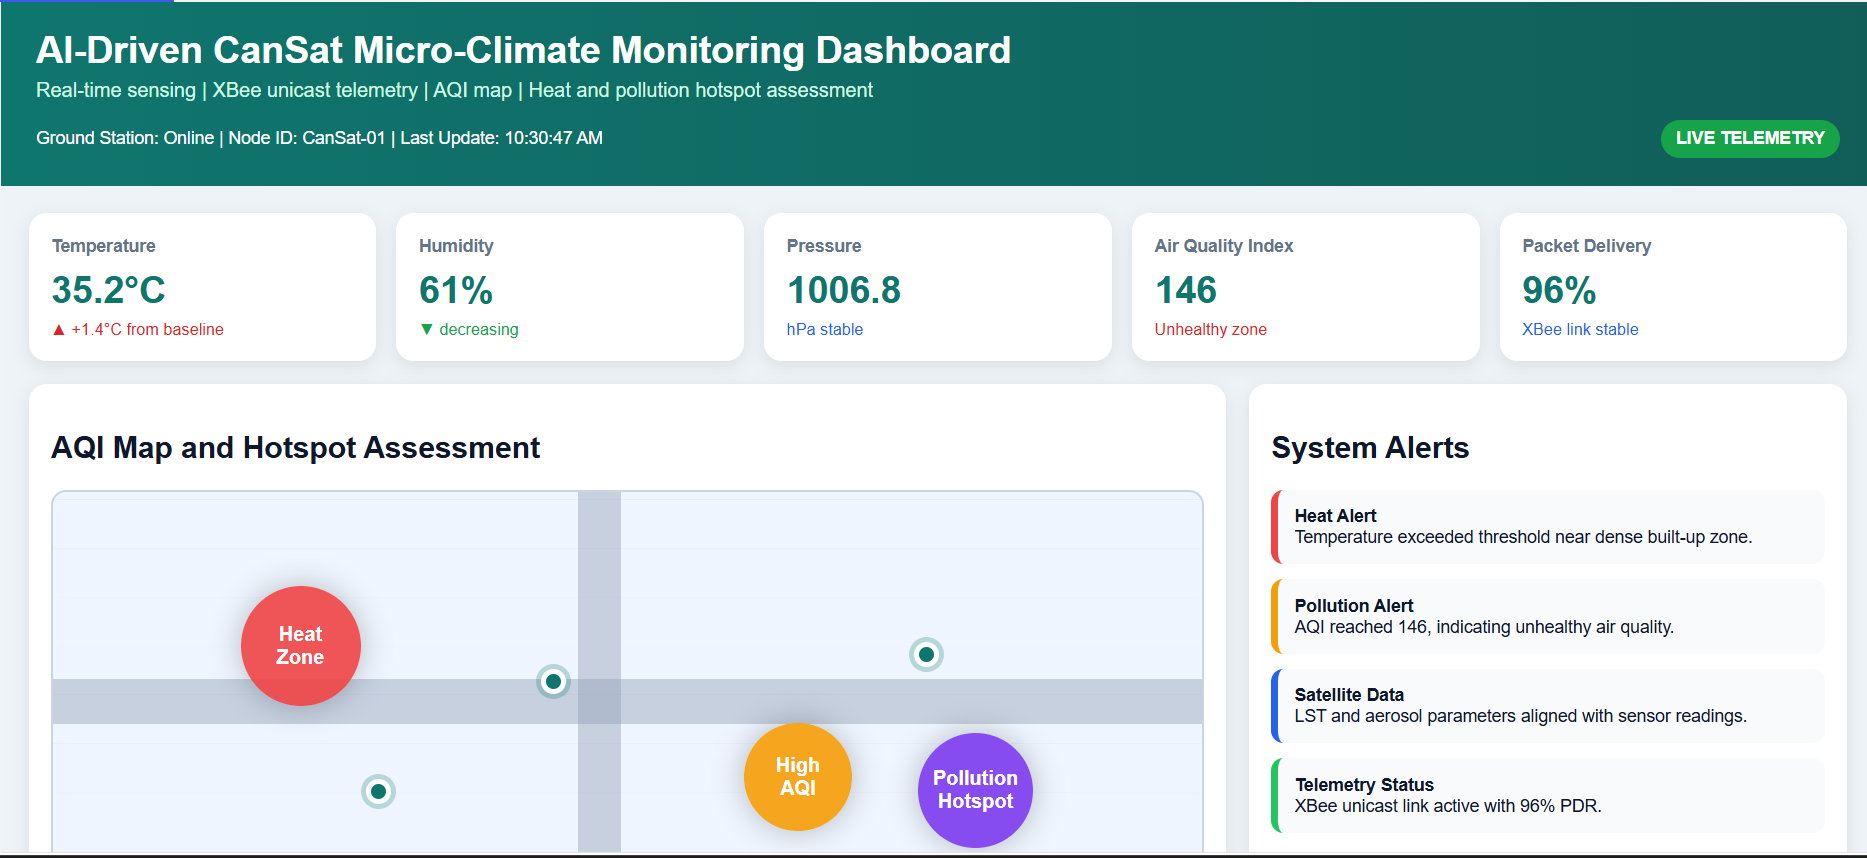
\includegraphics[width=0.97\linewidth]{dashboard.png}
\caption{Prototype dashboard showing real-time sensing, GPS-tagged telemetry, satellite-data synchronization, AQI mapping, hotspot assessment, AI-assisted status, system health, and communication performance.}
\label{fig:dashboard}
\end{figure*}

\vspace{0.3cm}

\subsection{Communication Performance Analysis}

To assess the system's performance for communication at varying distances, we adopted the metric packet delivery ratio (PDR). Telemetry efficiency has proven constant in experiments.

\begin{table}[!t]
\centering
\caption{XBee Communication Performance Evaluation}
\label{tab:pdr}
\renewcommand{\arraystretch}{1.2}
\begin{tabular}{|c|c|c|}
\hline
\textbf{Distance} & \textbf{PDR (\%)} & \textbf{Link Status} \\
\hline
100 m & 98 & Stable \\
300 m & 97 & Stable \\
500 m & 96 & Stable \\
700 m & 95 & Moderate \\
1 km & 94 & Acceptable \\
\hline
\end{tabular}
\end{table}

The findings show that the XBee-based unicast communication system can maintain reliable telemetry transmission over urban operating distances. It can also support low-power environmental sensing applications.

\vspace{0.3cm}

\subsection{Environmental Monitoring Results}

A prototype deployment that collected environmental observations shows detectable changes in temperature and air-quality conditions in the monitored urban environment. The experimental findings illustrate that temperature and AQI levels increase during peak monitoring periods, demonstrating the capability of the proposed framework to capture urban micro-climate variations.

The hotspot-assessment visualization also discovered areas linked with high environmental risk situations such as high-temperature zones and pollution concentration areas. The observation shows that localized sensing, satellite-assisted environmental context, and AI-assisted monitoring can all be combined for urban environments.

\begin{figure}[!t]
\centering
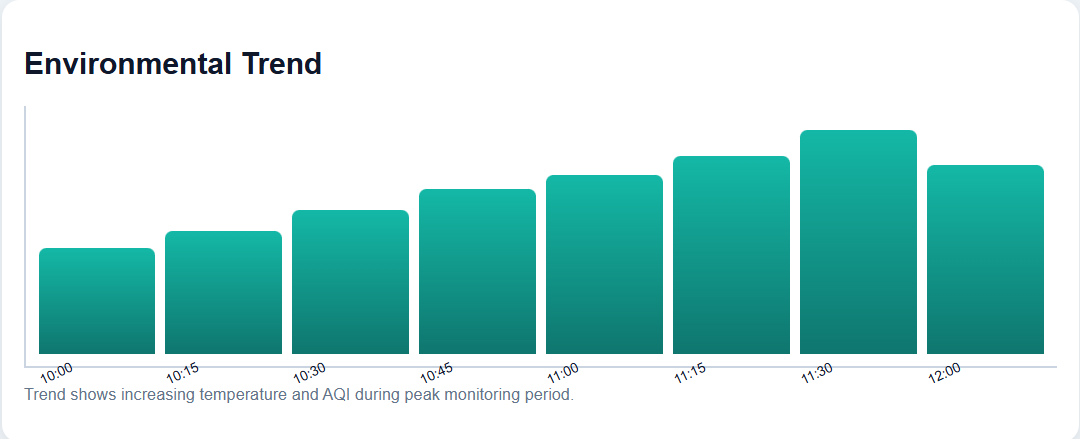
\includegraphics[width=\linewidth]{trend_graph.png}
\caption{Environmental trend visualization showing temporal variation in temperature and AQI during monitoring operations.}
\label{fig:trend}
\end{figure}

\vspace{0.3cm}

\subsection{System Validation and Discussion}

The prototype built can integrate environmental sensing, wireless telemetry, synchronization with satellite data, AI-assisted analysis and visualization in a unified deployable system successfully.

\begin{figure}[!t]
\centering
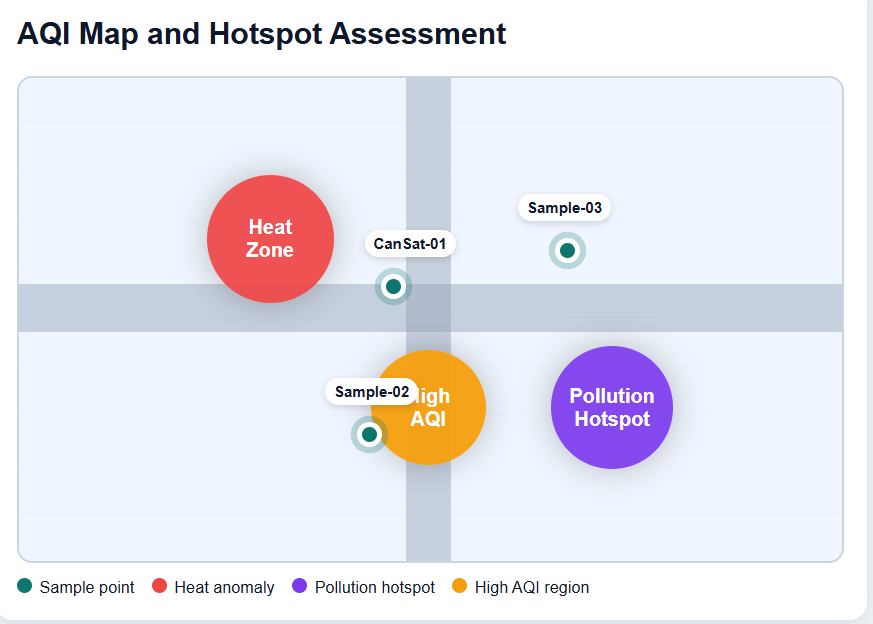
\includegraphics[width=\linewidth]{aqi_hotspot_map.png}
\caption{AQI map and hotspot-assessment interface showing localized heat anomalies, pollution hotspots, and environmental sample points within the monitored urban region.}
\label{fig:aqi_hotspot}
\end{figure}

The AQI-mapping and hotspot-assessment part of the developed monitoring dashboard is shown in Fig.~\ref{fig:aqi_hotspot}. Visualization layer detects specific environmental anomalies like hot spots, high AQI areas, pollution hot spots etc. using environmental observations that have been processed. To represent the ability to sense in a localized fashion throughout space, as well as to represent micro climate differences across the monitored urban space, multiple sensing nodes and environmental sample points are additionally shown.

The proposed architecture can serve mobile environmental monitoring, unlike conventional fixed environmental monitoring systems, which cannot provide mobile environmental monitoring. The use of sensor-based monitoring enhanced with satellite-aided invironmental context improves situational awareness of the environment and hotspot assessment capability.

The experimental implementation validates the practical applicability of the enhance framework for urban micro-climate monitoring applications. In addition, the results of the prototypes show that the system is capable of monitoring the environment on a scalable basis and future urban-climate intelligent platforms.

\begin{figure}[!t]
\centering
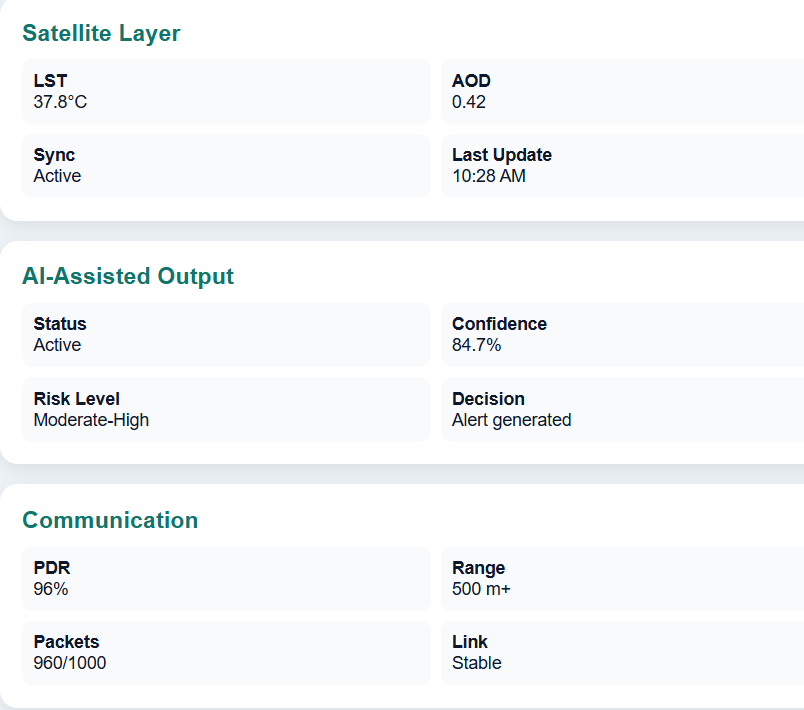
\includegraphics[width=0.9\linewidth]{ai_satellite_comm.png}
\caption{Satellite-data integration, AI-assisted analysis, and communication-status interface of the proposed CanSat-based monitoring framework.}
\label{fig:ai_satellite_comm}
\end{figure}

Fig.~\ref{fig:ai_satellite_comm} shows the components of the developed dashboard including synchronization of the satellite data, AI to analyze the environment, and communication-monitoring. The interface shows the parameters derived from the satellite data, such as land surface temperature (LST) and aerosol optical depth (AOD), as well as the synchronization status and update information. The AI-assisted analysis module offers environmental risk assessment, confidence indicators, automated decision supporting outputs for hotspot detection. In addition, the communication-monitoring section displays the reliability data of telemetry, such as packet delivery ratio (PDR), communication range, packet statistics and wireless-link stability data when the prototype operates.

\section{Conclusion}

A CanSat-based urban monitoring Framework using AI for microclimates has been presented in this study complemented with sensors, connectivity, satellite data and machine learning.  The proposed system uses a small and portable CanSat platform to allow real-time collection of environmental parameters including temperature, humidity, pressure and air quality.

XBee's unicast communication over a practical urban range with a delivery ratio of 94\%-97\% proves its reliability. Combining the ecological data collected by satellites with the information from monitoring took better readings of the urban situation. As a result, ingesting satellite-data into the AI system streamline pollution analysis for better and outreach to hotspots as well as can identify other environmental anomalies.

Based on experimental results, the proposed system provides a more economical and scalable solution for identifying hyperlocal environmental changes, with superior spatial resolution compared to existing fixed monitoring systems. The architecture and techniques of the framework demonstrate how sensing, communication and smart analytics can be integrated into one system.

Future works would include extending the system to work in a multi-node configuration, use mesh connectivity to provide coverage over a larger area, and enhancing the AI model with advanced learning to improve forecast accuracy. Strengthening the identification and management of urban risks will enable efficient use of ICTs for smart city efforts Management of urban environment and sustainable urbanization.

\section*{Acknowledgment}

The authors would like to thank United International University for providing the research environment and support.

\begin{thebibliography}{00}
\bibitem{p1} H. Du, F. Zhou, C. Li, W. Cai, H. Jiang, and Y. Cai, ``Analysis of the impact of land use on spatiotemporal patterns of surface urban heat island in rapid urbanization, a case study of Shanghai, China,'' \textit{Sustainability}, vol. 12, no. 3, p. 1171, 2020.
\bibitem{p2} T. Ara\'{u}jo, L. Silva, and A. Moreira, ``Evaluation of low-cost sensors for weather and carbon dioxide monitoring in internet of things context,'' \textit{IoT}, vol. 1, no. 2, pp. 286--308, 2020.
\bibitem{p3} C. Chun, M. H. Tanveer, and S. Chakravarty, ``The CanSat compendium: A review of scientific CanSats,'' \textit{Machines}, vol. 11, no. 7, p. 675, 2023.
\bibitem{p4} M. Elbestar, S. G. Aly, R. Ghannam, and H. Eraqi, ``AirFusion: sensor data fusion for air quality monitoring,'' \textit{Int. J. Remote Sens.}, pp. 1--24, 2025.
\bibitem{p5} M. S. Alam et al., ``Towards Green and Climate-Resilient Urbanization in Rajshahi City,'' \textit{Chinese J. Urban Environ. Stud.}, vol. 13, no. 01, p. 2550001, 2025.
\bibitem{R1} K. Fujiwara, M. Khomiakov, W. Yap, M. Ignatius, and F. Biljecki, ``Microclimate Vision: Multimodal prediction of climatic parameters using street-level and satellite imagery,'' \textit{Sustain. Cities Soc.}, vol. 114, p. 105733, 2024.
\bibitem{R3} L. R. Rodriguez, J. S. Ramos, and S. A. Dominguez, ``Simplifying the process to perform air temperature and UHI measurements at large scales,'' \textit{Sustain. Cities Soc.}, vol. 95, p. 104614, 2023.
\bibitem{R6} Q. Li, W. Wang, X. Luo, and J. Chen, ``Assessing built microclimate with building group frontal projection maps,'' \textit{Build. Environ.}, vol. 250, p. 111186, 2024.
\bibitem{R7} J. Han, A. Chong, J. Lim, S. Ramasamy, N. H. Wong, and F. Biljecki, ``Microclimate spatio-temporal prediction using deep learning and land use data,'' \textit{Build. Environ.}, vol. 253, p. 111358, 2024.
\bibitem{R8} M. Gubler, A. Christen, J. Remund, and S. Br\"{o}nnimann, ``Evaluation and application of a low-cost measurement network to study intra-urban temperature differences during summer 2018 in Bern, Switzerland,'' \textit{Urban Clim.}, vol. 37, p. 100817, 2021.
\bibitem{R11} A. Lefevre, B. Malet-Damour, H. Boyer, and G. Rivi\`{e}re, ``Advancing urban microclimate monitoring: the development of an environmental data measurement station using a low-tech approach,'' \textit{Sustainability}, vol. 16, no. 7, p. 3093, 2024.
\bibitem{R14} V. Shandas, J. Voelkel, J. Williams, and J. Hoffman, ``Integrating satellite and ground measurements for predicting locations of extreme urban heat,'' \textit{Climate}, vol. 7, no. 1, p. 5, 2019.
\bibitem{R15} Y. Pan, T. Morimoto, and T. Ichinose, ``Combining Multi-Source Satellite Data with a Microclimate Model to Analyze the Microclimate of an Urban Park,'' \textit{Climate}, vol. 12, no. 12, p. 197, 2024.
\bibitem{R16} D. Zhou et al., ``Satellite remote sensing of surface urban heat islands: Progress, challenges, and perspectives,'' \textit{Remote Sens.}, vol. 11, no. 1, p. 48, 2018.
\bibitem{R17} P. Pathak, P. Pandya, S. Shukla, A. Sane, and R. Sengupta, ``A sensor placement strategy for comprehensive urban heat island monitoring,'' \textit{ISPRS Int. J. Geo-Inf.}, vol. 12, no. 1, p. 11, 2022.
\bibitem{R18} L. Liang, J. Daniels, C. Bailey, L. Hu, R. Phillips, and J. South, ``Integrating low-cost sensor monitoring, satellite mapping, and geospatial artificial intelligence for intra-urban air pollution predictions,'' \textit{Environ. Pollut.}, vol. 331, p. 121832, 2023.
\bibitem{R21} A. Wang, S. Mora, Y. Machida, P. deSouza, S. Paul, O. Oyinlola, F. Duarte, and C. Ratti, ``Hyperlocal environmental data with a mobile platform in urban environments,'' \textit{Sci. Data}, vol. 10, no. 1, p. 524, 2023.
\bibitem{R22} O. Alsamrai, M. D. Redel-Macias, and M. P. Dorado, ``Real-time intelligent monitoring of outdoor air quality in an urban environment using IoT and machine learning algorithms,'' \textit{Appl. Sci.}, vol. 15, no. 16, p. 9088, 2025.
\bibitem{x5} K. Fujiwara, M. Khomiakov, W. Yap, M. Ignatius, and F. Biljecki, ``Microclimate Vision: Multimodal prediction of climatic parameters using street-level and satellite imagery,'' \textit{Sustain. Cities Soc.}, vol. 114, p. 105733, 2024.
\bibitem{x6} L. R. Rodriguez, J. S. Ramos, and S. A. Dominguez, ``Simplifying the process to perform air temperature and UHI measurements at large scales,'' \textit{Sustain. Cities Soc.}, vol. 95, p. 104614, 2023.
\bibitem{x7} Q. Li, W. Wang, Z. Yu, and J. Chen, ``Assessing urban micro-climates with vertical and horizontal building morphological cutting deep transfer learning neural networks,'' \textit{Build. Environ.}, vol. 234, p. 110186, 2023.
\bibitem{x8} J. Han, A. Chong, J. Lim, S. Ramasamy, N. H. Wong, and F. Biljecki, ``Microclimate spatio-temporal prediction using deep learning and land use data,'' \textit{Build. Environ.}, vol. 253, p. 111358, 2024.
\bibitem{x9} A. A. Scott, B. Zaitchik, D. W. Waugh, and K. O'Meara, ``Intraurban temperature variability in Baltimore,'' \textit{J. Appl. Meteorol. Climatol.}, vol. 56, no. 1, pp. 159--171, 2017.
\bibitem{x10} A. Lefevre, B. Malet-Damour, H. Boyer, and G. Rivi\`{e}re, ``Advancing urban microclimate monitoring: the development of an environmental data measurement station using a low-tech approach,'' \textit{Sustainability}, vol. 16, no. 7, p. 3093, 2024.
\bibitem{x11} F. Lyu, S. Wang, S. Y. Han, C. Catlett, and S. Wang, ``An integrated cyberGIS and machine learning framework for fine-scale prediction of Urban Heat Island,'' \textit{Urban Inform.}, vol. 1, no. 1, p. 6, 2022.
\bibitem{x12} L. Liang, J. Daniels, C. Bailey, L. Hu, R. Phillips, and J. South, ``Integrating low-cost sensor monitoring, satellite mapping, and geospatial artificial intelligence for intra-urban air pollution predictions,'' \textit{Environ. Pollut.}, vol. 331, p. 121832, 2023.
\bibitem{x13} R. E. Connolly et al., ``Long-term evaluation of a low-cost air sensor network for monitoring indoor and outdoor air quality at the community scale,'' \textit{Sci. Total Environ.}, vol. 807, p. 150797, 2022.
\bibitem{x14} V. R. Folifack Signing et al., ``IoT-based monitoring system and air quality prediction using machine learning for a healthy environment in Cameroon,'' \textit{Environ. Monit. Assess.}, vol. 196, no. 7, p. 621, 2024.
\bibitem{k1} Kaggle, ``Hourly Air Quality Index (AQI) of Bangladesh,'' Kaggle Dataset. [Online]. Available: https://www.kaggle.com/datasets/shakilofficial0/hourly-air-quality-index-aqi-of-bangladesh. Accessed: May 19, 2026.
\bibitem{k2} Kaggle, ``Dhaka Daily Air Quality and Weather Dataset,'' Kaggle Dataset. [Online]. Available: https://www.kaggle.com/datasets/albab12/dhaka-daily-air-quality-and-weather-dataset. Accessed: May 19, 2026.
\bibitem{k3} Kaggle, ``Urban Heat Island (UHI) Monitoring Dataset,'' Kaggle Dataset. [Online]. Available: https://www.kaggle.com/datasets/atharvasoundankar/urban-heat-island-uhi-monitoring-dataset. Accessed: May 19, 2026.
\end{thebibliography}

\vspace{12pt}
\color{red}
IEEE conference templates contain guidance text for composing and formatting conference papers. Please ensure that all template text is removed from your conference paper prior to submission to the conference. Failure to remove the template text from your paper may result in your paper not being published.

\end{document}
